\section{Oversampling to overcome class imbalance}
\label{sec:oversampling}

Class imbalance is a common problem in many machine learning tasks.
This is especially true in the case of the underrepresented classes being the most relevant ones, as is the case for the droplets in the vapour dataset.
The background label makes up \SI{99.914}{\percent} of all labeled pixels in the dataset, while the droplet border and droplet inside labels only make up \SI{0.063}{\percent} and \SI{0.023}{\percent} respectively.

Initially, this extreme unbalance made it impossible to train a model that could detect droplets and the mIoU would stagnate around \num{0.33}, which is the accuracy of a model that always predicts the background class.

One way to combat this imbalance is weighting the loss function of each class inversely proportional to the number of samples in the dataset that belong to that class, to prioritize predicting the underrepresented classes correctly during training. 
However, perhaps due to the unusually large imbalance, this method did not improve the performance of the model. Using smaller weights than the inverse distributions didn't achieve better results either.

The method that is applied in the thesis to overcome this problem is a form of \emph{oversampling}\cite{mohammedMachineLearningOversampling2020}, where the occurence of the underrepresented classes is artificially increased by showing the model samples that do contain these classes more often.
Although there are more sophisticated approaches to oversampling \cite{ReviewImbalancedData2017}, the solution used in this thesis is a simple one that is easy to implement, but has proven to be effective.

Since droplets are distributed very sparsely in the data, when splitting the images into smaller samples, a lot of the splits will not contain any droplets. 
Instead of including these empty regions in the training set, they are discarded when the split images are created.
Doing this changes the label distribution to \SI{99.84}{\percent} background, \SI{
0.116}{\percent} droplet border and \SI{0.044}{\percent} droplet inside, which doesn't appear to be much better than the original distribution, but roughly doubles the occurence rate of the droplet classes. 
This alone is enough to allow the model to learn to detect droplets with good accuracy.

To take this further, instead of splitting the image dimensions by two they could also be split by a larger factor, which would increase the relative density of droplets in the samples even more.
The results of this are shown in each experiment seperately, since the same split factor might not work well for all approaches.
No split factors larger than 4 were tested, since images would become very small and split droplets into different samples more often, which might also be detrimental. 

No further comparative studies were conducted to determine the optimal split factor or the best way to apply oversampling, since the results of this simple approach were already good enough to be used in the thesis.
Oversampling is used in all other experiments, since training on the vapour dataset is impossible without it.

\section{Mean Teacher for general improvement}
\label{sec:mean_teacher_general}

As described in \ref{sec:mean_teacher}, the mean teacher approach should enable us to utilize unlabeled data to improve the performance of our model.
To verify the effectiveness of this approach, the method is first tested on the Cityscapes dataset before it is applied to the vapour dataset.

In this experiment, the only concern is to improve the general performance of the model measured by the metrics described above. 
Further experiments will verify the effectiveness of the method for improving the generalization capabilities of the model on the vapour dataset.

\paragraph{Verification on Cityscapes} 

For the Cityscapes dataset training is done on images downsampled to a \qtyproduct{256 x 512}{\pixel} resolution. The initial learning rate is set to \num{1e-3} and the batch size to 16 containing 4 labeled and 12 unlabeled samples. The patience for the scheduler is set to 5 epochs and the reduction factor is set to \num{0.1}.
The weight of the consistency loss is ramped up to its maximum value of \num{1.0} over the first 15 epochs using a sigmoid ramp.
Consistency loss is calculated using the \emph{cross entropy loss} between the predictions of the student and the hard predictions of the teacher (meaning after applying \emph{argmax}).
The teacher is updated using an EMA with a decay $\alpha$ of \num{0.996}.

For the baseline model, the best results are achieved by using an initial learning rate of \num{1e-4} with a batch size of 16, a scheduler patience of 20 epochs and a reduction factor of \num{0.5}. 

The baseline model is trained on 100 labeled samples from the training set, while the mean teacher model is trained on the same 100 lableled samples plus all other samples from the training set as unlabeled samples.
A training epoch when using MT is considered to be finished when the model has seen all unlabeled samples once, with the labeled samples being seen as many times as necessary to fill the batch size. This means epochs for MT training contain considerably more samples than epochs for baseline training, which is why the patience value for baseline training is higher.

For the baseline model, the augmentation pipeline consists of a random \numproduct{224 x 224} crop, a random translation, scaling and rotation with a probability of \num{0.5}, a RGB-shift with a probability of \num{0.5} and a random variation of the image brightness and contrast with a probability of \num{0.5}.  

The augmentation pipeline for the MT training employs a different set of augmentations, since strong asymmetrical augmentations between teacher and student are important for the MT approach to properly function. For this, the augmentation pipeline is inspired by \Citeauthor{schererPseudoLabelNoiseSuppression2022}\cite{schererPseudoLabelNoiseSuppression2022}. It contains the same shift, scale, rotation and crop operations as the baseline augmentations, but also applies a strong dropout of \num{0.5} to the student model, as well as using a \emph{CowMask} technique to compose new samples by combining two images as well as their teacher predictions.
For this technique a mask such as the one shown in Figure \ref{fig:cowmask} is generated and applied to an image and its pseudo label. The same is done for a second image and its pseudo label with the inverted mask and both are combined.

Finally, the images are normalized using the mean and standard deviation of the ImageNet dataset in both baseline and MT training.

\begin{figure}[htbp]
    \centering
    \makebox[\textwidth][c]{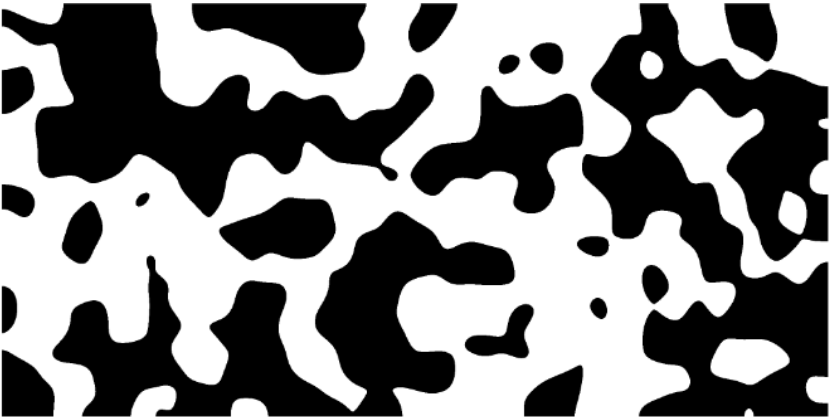
\includegraphics[width=0.4\textwidth]{images/Screenshot-20230221170853-829x417.png}}
    \vspace{0.1cm}
    \caption{Example for a cow mask used in the training process. The white areas mark regions that use the first image, while the black areas use the second image. From \cite{schererPseudoLabelNoiseSuppression2022}}
    \label{fig:cowmask}
\end{figure}

\paragraph{Results on Cityscapes}
With the MT approach, the model is able to achieve a mean IoU of \num{0.426} on the validation set, which is a significant improvement over the baseline model with a mean IoU of \num{0.349}.

However, this improvement is only achievable within a very small space of hyperparameters, as all training runs with different hyperparameters than described above yielded worse results than even the baseline model.

This deterioration in performance can likely be attributed to very poor pseudo label quality. As \citeauthor{schererPseudoLabelNoiseSuppression2022}\cite{schererPseudoLabelNoiseSuppression2022} discovered in their analysis of \emph{pseudo label filtering} techniques, pseudo labels with poor quality have a detrimental effect on final model performance.
Since the setup used in this thesis doesn't achieve very high performance on the Cityscapes dataset as is, even when using all labeled samples (mIoU of \num{0.475}), it stands to reason that label quality may hurt the training process if hyperparameters are suboptimal.

Nonetheless, the results of this experiment show that the MT approach is able to improve the performance of the model. With the supervised performance on the target dataset being signifcantly better than on the Cityscapes dataset, it is likely that the MT approach will be able to improve the performance of the model on the vapour dataset as well.

For a more comprehensive overview of training results, see Table \ref{tab:cityscapes_results_mt}.

\begin{table}[htbp]
    \centering
    \begin{tabular}{llllllllrr}
        \toprule
        \multicolumn{9}{l}{Cityscpapes Training}\\  
        \midrule
        Approach & \#lbls & lr & bsize & lrsf & lrsp & Dropout & $\alpha$ & Loss &
        mIoU \\
        \midrule 
        Baseline & all & $0.0001$ & $16$ & $0.5$ & $10$ & - & - & $0.216$ & $0.475$ \\
        MT & 100 & $0.001$ & $16$ & $0.1$ & $5$ & \num{0.5} & \num{0.996} & $0.644$ & $\mathbf{0.426}$ \\
        MT & 100 & $0.001$ & $16$ & $0.1$ & $5$ & \num{0.4} & \num{0.996} & $0.559$ & $0.412$ \\
        Baseline & 100 & $0.0001$ & $16$ & $0.5$ & $30$ & \num{0.2} & - & $0.444$ & $0.349$ \\
        Baseline & 100 & $0.0001$ & $16$ & $0.5$ & $30$ & - & - & $0.469$ & $0.331$ \\
        \bottomrule
    \end{tabular}
    \vspace{0.1cm}
    \caption{The best training results of the Mean Teacher approach on the Cityscapes dataset, as well as the supervised baseline performance along with important hyperparameters. For abbreviations refer to Table \ref{tab:abbreviations}.}
    \label{tab:cityscapes_results_mt}
\end{table}

\paragraph{Setup on vapour dataset}
The training setup for the vapour dataset is very similar to the Cityscapes setup, with the images being split in half along the vartical and horizontal axis and these 4 segments being used as seperate samples. The decision to split the images instead of resizing them was made because the relevant objects in the images are already quite small, so resizing them might make it impossible to detect some of them. This leaves us with \qtyproduct{640 x 512}{\pixel} images, which necessitated lowering the batch size to 12 for baseline training and 8 (2 labeled, 6 unlabeled) for MT training.
Learning rate was generally found to be optimal around \num{1e-3}.

Another difference in the setup is the augmentation pipeline, which is similar to the Cityscapes pipeline, but replaces the RGB-shift with gaussian noise, since the vapour dataset contains greyscale images. The gaussian noise might also be able to mimic some of the noise the camera produces, so it seems like an adequate replacement.
Furthermore, we also explore using \emph{CutMix}\cite{yunCutMixRegularizationStrategy2019} for mixing pseudo labels instead of the CowMask technique used for Cityscapes. 
CutMix cuts a rectangular region of the image instead of the varying sizes of blobs in the CowMask technique.
The reason this may be more suitable to the vapour dataset is that the objects in the images are generally quite small, so the CowMask technique, which masks generally smaller regions might not be effective in combining relevant features from the two images. On Cityscapes, CutMix was not attempted since \Citeauthor{schererPseudoLabelNoiseSuppression2022}\cite{schererPseudoLabelNoiseSuppression2022} already concluded that the CowMask technique was superior.

\paragraph{Results on vapour dataset}


\section{Mean teacher for generalization}
\label{sec:generalization}

Another hope for the MT approach is that it will be able to improve the generalization capabilities of the model. Since different imaging parameters or different SAW devices will produce slightly different images, being able to adapt the model to new parameters without having to label new data would be a huge advantage.

To explorer this, two subsets (S1 and S2) of the vapour datasets with different parameters are used to create two new datasets (DS1 and DS2). DS1 contains the labeled samples from S1 as well as all samples from S2 with the labels removed. DS2 is built in the same way, but with S2 as the labeled dataset and S1 as the unlabeled dataset.

The model is then trained on one of the two datasets (DS1 or DS2) and evaluated on the validation set of the other dataset (DS2 or DS1), once with only the labeled samples and once with the unlabeled samples using MT. This is repeated for both datasets, so that one model is trained on either dataset. 

To avoid adapting the model purely to one subset, the test set is used for validation during training. 

If including the unlabeled samples from S2 helps the model improve on the test set of S2 compared to only having seen the labeled samples from S1 (and vice versa), it would indicate that the MT method does indeed help the model generalize without new labeled data.

Training parameters are the same as in \ref{sec:mean_teacher_general}.

\paragraph{Results}


\section{Binary instead of multi-class segmentation}
\label{sec:binary}

In \ref{sec:algorithm} it's stated that training the model to segement the image into three different classes helps to filter out common model errors in later stages of the measurement algorithm. 
However, introducing a third class also makes the problem more difficult to learn. It could be that training the model on only two classes (background and in-focus droplet) would enable the model to avoid the errors in the first place, since it can learn the criterium for a droplet bein in focus more easily.

To test this, the model is trained on the vapour dataset, but with all different droplet labels combined into a single class. The model is then evaluated on the test set that underwent the same transformation. 

During the evaluation process, the filtering step performed by the droplet measurement algorithm is obviously skipped, since the inside labels don't exist anymore. 

Training parameters are the same as in \ref{sec:mean_teacher_general}.

\paragraph{Results}


\section{Training with reduced layers}
\label{sec:reduced_layers}

The architecture of the model presented in chapter \ref{sec:architectures} has five distinct downsampling and upsampling stages in its encoder and decoder paths respectively.
The stated purpose of the lower layers is to be able to utilize more contextual information since neurons in lower layers have a wider \emph{receptive field} than neurons in higher layers.

However, for our specific problem, objects are generally quite small  and the problem itself isn't very complex, so the contextual information provided by the lower layers might not be as useful as it is for larger objects.
Additionally, including the lower layers may not only be unneccessary, but also detrimental to the performance of the model, since it increases the number of parameters and with that the computational complexity of the model, which makes it harder to train. 
This also plays a role in the demand for computational resources during training and inference, since even only omitting the deepest layers reduces the trainable parameter count from 24.5\,M to 9.1\,M.

To explore this hypothesis, the model is trained on the vapour dataset with the encoder and decoder paths reduced to only three stages each besides the input and output stage (final encoder stride is 8 instead of 16). The model is then evaluated as normal.

Because of time constraints, pretraining the reduced model on the Cityscapes dataset was not attempted, however since the Cityscapes dataset is much more complex than our own, it is unlikely the model would have achieved good results on it in the first place.

The experiment compares the performance with and without semi supervised learning, with a split factor of 2.

Training parameters are the same as in \ref{sec:mean_teacher_general}.

\paragraph{Results}